\documentclass[12pt,a4paper]{report}

% ---------------------------------------------------------------------------
% Trustworthy Agentic AI for Intent-Based Self-Healing SDN
% Semester report -- IIIT Bangalore, Department of Computer Science
% ---------------------------------------------------------------------------

\usepackage[T1]{fontenc}
\usepackage[utf8]{inputenc}
\usepackage[a4paper,top=1in,bottom=1in,left=1.25in,right=1.25in]{geometry}
\usepackage{graphicx}
\usepackage{float}
\usepackage{booktabs}
\usepackage{array}
\usepackage{tabularx}
\usepackage{longtable}
\usepackage{amsmath}
\usepackage{amssymb}
\usepackage{xcolor}
\usepackage{caption}
\usepackage{enumitem}
\usepackage{fancyhdr}
\usepackage{hyperref}
\usepackage{tikz}
\usetikzlibrary{arrows.meta,positioning,shapes.geometric,fit,backgrounds}

\hypersetup{
    colorlinks=true,
    linkcolor=blue!50!black,
    citecolor=blue!50!black,
    urlcolor=blue!50!black,
    pdftitle={Trustworthy Agentic AI for Intent-Based Self-Healing SDN},
    pdfauthor={Kamal Nayan Kumar, Altaf Raja, Ankit Kumar Keshari, Soumya Nimje}
}

% Colours used throughout, mirroring the dashboard palette.
\definecolor{sdnblue}{HTML}{2D6BE4}
\definecolor{sdnred}{HTML}{DC2626}
\definecolor{sdnamber}{HTML}{B45309}
\definecolor{sdngreen}{HTML}{059669}
\definecolor{sdngrey}{HTML}{5A6472}

% ---------------------------------------------------------------------------
% Footer.
%
% The college logo appears on the title page only; body pages carry a plain
% running footer with the report title and page number.
% ---------------------------------------------------------------------------
\pagestyle{fancy}
\fancyhf{}
\renewcommand{\headrulewidth}{0pt}
\renewcommand{\footrulewidth}{0.4pt}

\fancyfoot[C]{%
    \footnotesize
    \textbf{Trustworthy Agentic AI for Intent-Based Self-Healing SDN}
    \hfill Page \thepage{} of \pageref{LastPage}%
}

% Title page keeps the logo at the bottom instead of the running footer.
\fancypagestyle{titlepage}{%
    \fancyhf{}
    \renewcommand{\headrulewidth}{0pt}
    \renewcommand{\footrulewidth}{0pt}
    \fancyfoot[C]{%
        \IfFileExists{logo.jpeg}{%
            \raisebox{0.45cm}{\includegraphics[height=1.9cm]{logo.jpeg}}%
        }{}%
    }
}

\usepackage{lastpage}

% fancyhdr asks for a little more clearance between the text block and the
% footer so the logo does not crowd the last line.
\setlength{\footskip}{36pt}

% ---------------------------------------------------------------------------
% Table helpers
% ---------------------------------------------------------------------------
\newcolumntype{L}[1]{>{\raggedright\arraybackslash}p{#1}}
\newcolumntype{C}[1]{>{\centering\arraybackslash}p{#1}}
\newcommand{\tblhead}[1]{\textbf{\textcolor{sdnblue}{#1}}}

% Node names like `observe_after` are long monospace tokens in narrow table
% cells. Allow them to break rather than overflowing the column.
\usepackage{seqsplit}

\setlength{\parskip}{4pt}
\setlist[itemize]{leftmargin=1.5em,itemsep=2pt,topsep=3pt}
\setlist[enumerate]{leftmargin=1.8em,itemsep=2pt,topsep=3pt}

% ---------------------------------------------------------------------------
% Document
% ---------------------------------------------------------------------------
\begin{document}

% ============================ TITLE PAGE ==================================
\begin{titlepage}
\thispagestyle{titlepage}
\centering

\vspace*{1.0cm}

{\Huge\bfseries Trustworthy Agentic AI for\\[6pt]
 Intent-Based Self-Healing SDN}\\[10pt]
{\large A LangGraph Agent that Decides When \emph{Not} to Act\par}

\vspace{1.1cm}

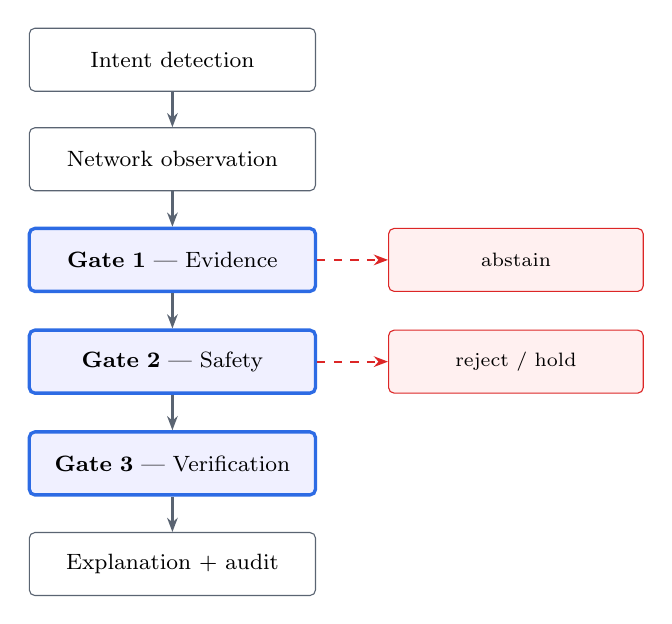
\begin{tikzpicture}[
    node distance=4.5mm and 7mm,
    box/.style={draw=sdngrey, rounded corners=2pt, minimum height=8mm,
                text width=34mm, align=center, font=\footnotesize, fill=white},
    gate/.style={box, draw=sdnblue, very thick, fill=blue!6},
    term/.style={box, draw=sdnred, fill=red!6, text width=30mm, font=\scriptsize},
    ar/.style={-{Stealth[length=1.8mm]}, thick, draw=sdngrey}
]
% The happy path is a single column so it fits the title page comfortably; the
% two refusal branches leave to the right.
\node[box] (intent) {Intent detection};
\node[box, below=of intent] (obs) {Network observation};
\node[gate, below=of obs] (g1) {\textbf{Gate 1} --- Evidence};
\node[gate, below=of g1] (g2) {\textbf{Gate 2} --- Safety};
\node[gate, below=of g2] (g3) {\textbf{Gate 3} --- Verification};
\node[box, below=of g3] (out) {Explanation + audit};

\node[term, right=9mm of g1] (abstain) {abstain};
\node[term, right=9mm of g2] (reject) {reject / hold};

\draw[ar] (intent) -- (obs);
\draw[ar] (obs) -- (g1);
\draw[ar] (g1) -- (g2);
\draw[ar] (g2) -- (g3);
\draw[ar] (g3) -- (out);
\draw[ar, dashed, draw=sdnred] (g1.east) -- (abstain.west);
\draw[ar, dashed, draw=sdnred] (g2.east) -- (reject.west);
\end{tikzpicture}

\vspace{1.2cm}

{\large\textbf{Submitted by}}\\[6pt]
\begin{tabular}{@{}l@{\hspace{1.2cm}}l@{}}
Kamal Nayan Kumar      & 23BDS026 \\
Altaf Raja             & 23BCS011 \\
Ankit Kumar Keshari    & 23BCS015 \\
Soumya Nimje           & 23BEC054 \\
\end{tabular}

\vfill

{\large\textbf{Under the Guidance of}}\\[6pt]
{\Large\textbf{Dr.\ Jagadeesha R\,B}}\\[2pt]
{\large Course Instructor}\\[10pt]

{\small Progress Report \quad\textbar\quad Academic Year 2025--26\par}

% Clearance for the logo, which this page alone carries in its footer.
\vspace{2.5cm}
\end{titlepage}

% ============================ ABSTRACT ====================================
\begin{abstract}
\noindent
Software-Defined Networking gives a network administrator precise programmatic
control over traffic paths, but it does not tell them \emph{when} to use that
control, nor whether a change actually helped. This project builds a working
local system that closes that gap: an administrator states a performance goal
in ordinary language, and an agent built on LangGraph either restores the
network, explains precisely why it declined to act, or reports that recovery
failed --- and every one of those outcomes is grounded in a measurement taken
from a real OpenFlow network rather than inferred.

The central design decision is that the LLM is not trusted with the decision to
change the network. It is used only to parse intent, narrate evidence and write
the final explanation. Three deterministic gates stand between the model's
suggestion and the data plane: an \textbf{evidence} gate that refuses to act on
missing or stale measurements, a \textbf{safety} gate that validates every
mutation against an explicit constraint set, and a \textbf{verification} gate
that re-measures the network afterwards and reports failure when the intent is
still unmet. A successful command is never reported as a successful recovery.

The system runs entirely on one machine against a Mininet topology of four
hosts and four OpenFlow switches driven by a Ryu controller, with a dashboard
streaming live telemetry over Server-Sent Events. Evaluation over the video
latency scenario shows the agent correctly distinguishing a healthy network
(\texttt{intent\_satisfied}, no change made) from a genuinely violated one, and
correctly rerouting onto a congestion-free path while reporting the recovery as
failed when latency did not actually improve.
\end{abstract}

\tableofcontents
\newpage

% ============================ 1. INTRODUCTION =============================
\section{Introduction and Problem Statement}

\subsection{Background}

A traditional network is managed by rules written by people: static routes,
threshold alarms, and manual intervention when something looks wrong. This works
until traffic changes faster than operators can re-plan. Software-Defined
Networking (SDN) changes the arrangement by separating the \emph{control plane}
--- where routing decisions are made --- from the \emph{data plane} --- where
packets are actually forwarded. A central controller programs forwarding tables
into every switch through the OpenFlow protocol, so a traffic path can be
changed across the whole network in milliseconds rather than by touching devices
one at a time.

That power creates its own problem. SDN gives an administrator the \emph{ability}
to reroute traffic, but it says nothing about \emph{when} rerouting is the right
response, or whether the change actually improved anything. Worse, it makes
mistakes cheap to make and expensive to detect: a well-meaning reroute can send
traffic through a worse path, disturb a critical flow, or break connectivity
entirely --- and the system will happily report the command as successfully
executed.

\subsection{The Problem}

Consider an ordinary requirement. A company carries live video between two
sites and has promised its users that this video will always stay under
\textbf{50~ms}. One afternoon, an unrelated background transfer --- say a backup
job or a large file sync --- happens to traverse the same link the video uses.
That link becomes congested.

\begin{center}
\begin{tabular}{@{}p{0.92\linewidth}@{}}
\toprule
\textbf{What a human operator does:}
\quad\emph{``Video is slow. Let me check which link is busy\ldots\ move it to
the backup link\ldots\ did that work? Where is it going now? Is the voice call
still fine?''} \\
\bottomrule
\end{tabular}
\end{center}

Every step of that reasoning is a decision made under uncertainty. The operator
is guessing from partial data, and critically, \textbf{there is no automatic
check that the guess was correct}. A reroute that appears to succeed but pushes
latency from 120~ms to 140~ms looks identical to one that genuinely fixed the
problem, unless something measures the result afterwards.

A second, subtler failure mode: the operator may act when they should not. If a
single latency reading happens to fall just under the threshold, a system that
trusts that reading will conclude ``no problem'' and do nothing --- while the
true behaviour is that the flow oscillates above and below the limit and the
user's video is still dropping frames.

\subsection{Why an LLM Alone Is Not the Answer}

Large language models are naturally suited to the fuzzy parts of this task. They
can read ``optimise the video latency and keep it under 50~ms'' and turn it into
a structured goal. They can explain a diagnosis in language an operator
understands. What they cannot do is be \emph{trusted} with a decision that
affects a running network. A language model may hallucinate a measurement that
was never taken, assert that a path is safe without checking, or state that a
change succeeded when nothing verified it. Prompting a model to ``be careful''
does not make it careful.

\subsection{Our Approach}

This project builds an agent that is genuinely useful \emph{and} genuinely
bounded. The LLM handles what it is good at; ordinary deterministic Python
handles everything that must not be improvised. Three gates stand between the
model and the network:

\begin{center}
\begin{tabular}{@{}p{0.92\linewidth}@{}}
\toprule
\textbf{The principle:} \emph{the agent may propose; only verified evidence
may decide.} \\
\bottomrule
\end{tabular}
\end{center}

Concretely, the system must:

\begin{enumerate}
    \item \textbf{Detect} a violated intent from real measurements.
    \item \textbf{Gather} trustworthy evidence and identify the bottleneck.
    \item \textbf{Decide} whether the evidence justifies acting at all --- and
          abstain if it does not.
    \item \textbf{Select} a permitted alternative path.
    \item \textbf{Validate} the action against explicit safety constraints.
    \item \textbf{Execute} it through the SDN controller.
    \item \textbf{Verify} by measuring again, and report the real outcome.
\end{enumerate}

Steps 3, 5 and 7 are the contribution. They are what separate this from a
prompt that asks a model to reroute traffic, and they are the reason the system
can be trusted to say \emph{``I did not do anything, and here is exactly why.''}

% ============================ 2. SOLUTION =================================
\section{Solution Approach}

\subsection{Design Principle}

The architecture follows from a single rule: \textbf{separate proposing from
deciding}. The LLM is a capable but fallible component, so it is confined to
tasks where a mistake is recoverable --- parsing language and writing prose. Any
decision that can damage the running network is made by ordinary deterministic
code that behaves identically every time.

\subsection{Step-by-Step Approach}

\paragraph{Step 1 --- Establish a real network to act on.}
Nothing can be verified against a simulation of a network, so the project builds
an actual Mininet topology: four hosts and four OpenFlow 1.3 switches connected
by a ring. A Ryu controller installs forwarding rules. Traffic generation,
latency measurement and packet counting all happen on real interfaces. The
entire lab runs inside its own network namespace so that experiment traffic can
never reach the machine's real network interfaces.

\paragraph{Step 2 --- Measure continuously.}
A telemetry collector samples the network on demand: it pings each flow to
obtain round-trip times, reads per-link byte counters from the switches, and
packages everything into a single coherent snapshot. Every number the system
acts on originates here, from the datapath, and nowhere else.

\paragraph{Step 3 --- Parse the intent.}
The administrator's sentence is converted into a structured intent --- source
host, destination, traffic class, and the numeric target --- using the LLM, with
a deterministic keyword parser as fallback when no API key is configured. The
system reports which of the two it used rather than implying the model was
involved when it was not.

\paragraph{Step 4 --- Assess the evidence (Gate 1).}
Before considering any change, the system checks that the measurements it needs
actually exist, are recent enough under the configured policy, and are
internally consistent. Three distinct outcomes are possible here and they are
never conflated:

\begin{center}
\begin{tabular}{@{}L{3.4cm}L{9.1cm}@{}}
\toprule
\textbf{Outcome} & \textbf{Meaning} \\
\midrule
\texttt{intent\_satisfied}
  & Measured and comfortably inside the target. A confident, correct no-op. \\
\texttt{abstained}
  & The evidence is missing, stale or inconclusive. A refusal to act. \\
\texttt{diagnose}
  & The intent is genuinely breached and the evidence supports acting. \\
\bottomrule
\end{tabular}
\end{center}

Collapsing these would be a serious error. Reporting \texttt{satisfied} when the
evidence is merely absent makes the agent look confident about a network it has
not measured; reporting \texttt{abstained} when the network is healthy makes a
working system look broken.

\paragraph{Step 5 --- Diagnose and enumerate alternatives.}
The agent identifies the likely bottleneck and asks the topology service for
every candidate path between the endpoints. Each candidate is scored, and one
important rule governs that scoring: \textbf{a path that crosses a congested
link is not a repair}. Routing traffic around a bottleneck is the entire point,
so crossing it is disqualifying rather than merely expensive. Among paths that
avoid congestion, accumulated delay decides.

\paragraph{Step 6 --- Validate the action (Gate 2).}
The chosen action passes nine deterministic checks: the operation is on an
allow-list, the endpoints exist, the path is well formed, the hop count is
within budget, every link on it is operational, capacity is respected, protected
flows are untouched, the action is scoped to the declared flow, and the request
has not expired or been duplicated. A statement from the model that an action is
safe carries no weight here; only the validator can approve it.

\paragraph{Step 7 --- Execute through the controller.}
Only an approved action reaches the controller, which installs OpenFlow rules for
the new path. This is the only point in the system where the network is
modified.

\paragraph{Step 8 --- Verify (Gate 3).}
The system measures the network again \emph{after} the change and compares the
fresh result against the intent. This step exists for one reason: \textbf{a
successful command is not a successful recovery}. A reroute can install
perfectly and change nothing, and a system that reports success there is lying
by omission. The gate distinguishes full recovery, partial improvement, failure,
and unverified.

\paragraph{Step 9 --- Explain and record.}
The run produces a human-readable explanation grounded in the numbers actually
measured, together with the full audit trail: which checks ran, which passed,
what was executed, and what the result was.

\subsection{What Makes This Trustworthy}

The trustworthiness argument is structural rather than a claim about model
behaviour:

\begin{itemize}
    \item The LLM has \textbf{no tool that mutates the network}. It cannot
          execute anything; it can only be invoked through a fixed allow-list,
          and the only mutating tool refuses to act on an unvalidated action.
    \item Every gate is \textbf{deterministic}. The same inputs always produce
          the same decision, with no model in the loop.
    \item \textbf{Unknown is never treated as healthy.} A missing measurement
          yields ``unknown'', never ``no violation''.
    \item \textbf{Failure is reportable.} The system has first-class outcomes
          for refusal, rejection and failed recovery, so it is never forced to
          claim success.
\end{itemize}

% ============================ 3. TECH STACK ===============================
\section{Technology Stack}

Everything except the optional external LLM API runs locally on the development
machine. No hosted services, no public endpoints.

\subsection{Frontend}

\begin{center}
\begin{tabular}{@{}L{3.2cm}L{2.8cm}L{7.8cm}@{}}
\toprule
\textbf{Technology} & \textbf{Version} & \textbf{Role} \\
\midrule
Next.js          & 16.4.0  & App framework and dev server (port 3000) \\
React            & 19.3.0  & User interface \\
TypeScript       & 5.9.3   & Static typing for telemetry payloads \\
CSS / Tailwind   & 4.3.3   & Styling \\
Playwright       & 1.64.0  & Browser end-to-end tests \\
\bottomrule
\end{tabular}
\end{center}

The topology view is drawn as hand-built SVG rather than pulled from a graph
library. This keeps the congested-link rendering and the live utilisation
encoding under direct control, which matters because the colour of a link is a
claim about network state.

\subsection{Backend}

\begin{center}
\begin{tabular}{@{}L{3.2cm}L{2.8cm}L{7.8cm}@{}}
\toprule
\textbf{Technology} & \textbf{Version} & \textbf{Role} \\
\midrule
Python           & 3.12.15 & Runtime \\
FastAPI          & 0.143.0 & HTTP and Server-Sent Events server \\
Uvicorn          & 0.54.0  & ASGI server (port 8000) \\
Pydantic         & 2.14.1  & Strict schemas for every payload \\
LangGraph        & 1.2.15  & Agent workflow as an explicit state graph \\
LangChain Core   & 1.6.10  & LLM interface used by the agent \\
SQLAlchemy       & 2.1.4   & Persistence models \\
Groq SDK         & 1.7.0   & Optional LLM access \\
Pytest           & 9.1.1   & Test framework \\
\bottomrule
\end{tabular}
\end{center}

Pydantic models are configured to \emph{forbid extra fields}. The lab may add
descriptive attributes freely, but the contract between components remains
exactly what the schema declares.

\subsection{Network Lab}

\begin{center}
\begin{tabular}{@{}L{3.2cm}L{2.8cm}L{7.8cm}@{}}
\toprule
\textbf{Technology} & \textbf{Version} & \textbf{Role} \\
\midrule
Mininet          & 2.3.0   & Topology, hosts and links \\
Ryu              & vendored & OpenFlow controller \\
of13switch.py    & custom  & User-space OpenFlow 1.3 switch \\
Eventlet         & 0.41.2  & Async runtime for the controller \\
\bottomrule
\end{tabular}
\end{center}

Because the Open vSwitch backend is not always available, the project ships a
pure-Python user-space OpenFlow switch. This makes the lab reproducible on any
Linux machine without kernel modules, at the cost of throughput: it saturates
near 40~Mbps, well below the 1~Gb/s links it emulates.

The lab runs inside an isolated network namespace and exposes its API over a
unix domain socket rather than TCP, so no network-control port is ever opened.

% ============================ 4. LANGGRAPH ================================
\section{LangGraph Agent Workflow}

The agent is expressed as an explicit state graph rather than a free-running
prompt. Every node has one job, state is typed, and the route between nodes is
decided by code rather than by the model.

\subsection{Graph Topology}

The diagram below is generated directly from the \texttt{graph.py} assembly:
every \texttt{add\_node} and \texttt{add\_edge} call is reflected exactly once.
Solid arrows are unconditional edges; dashed arrows carry the condition label
from the three routing functions.

\begin{figure}[htbp]
\centering
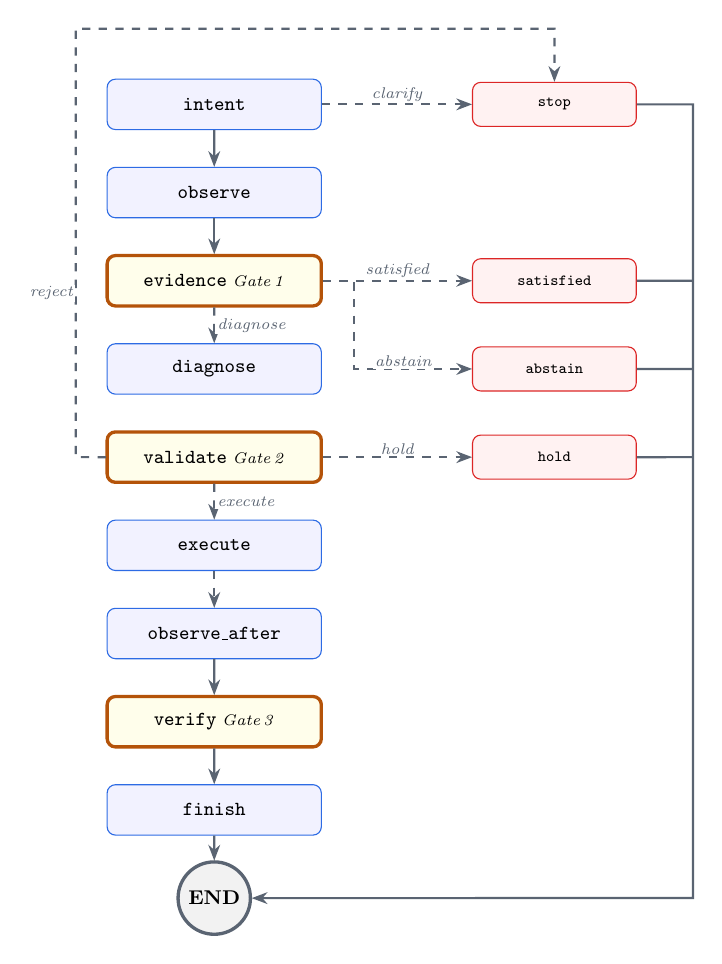
\begin{tikzpicture}[
  scale=0.8, transform shape,
  proc/.style={draw=sdnblue, rounded corners=3pt,
    minimum width=34mm, minimum height=8mm,
    align=center, font=\small, fill=blue!5},
  gate/.style={draw=sdnamber, very thick, rounded corners=3pt,
    minimum width=34mm, minimum height=8mm,
    align=center, font=\small, fill=yellow!8},
  term/.style={draw=sdnred, rounded corners=3pt,
    minimum width=26mm, minimum height=7mm,
    align=center, font=\scriptsize, fill=red!5},
  endnode/.style={draw=sdngrey, very thick, circle,
    minimum size=10mm, font=\small\bfseries, fill=gray!10},
  ar/.style={-{Stealth[length=2mm]}, thick, draw=sdngrey},
  cond/.style={-{Stealth[length=2mm]}, thick, dashed, draw=sdngrey},
  line/.style={thick, draw=sdngrey},
  elbl/.style={font=\scriptsize\itshape, text=sdngrey, fill=white, inner sep=1pt}
]

% ---- Happy-path column (x = 0), one fixed row per node ----
\node[proc]  (intent)      at (0,0)     {\texttt{intent}};
\node[proc]  (observe)     at (0,-1.4)  {\texttt{observe}};
\node[gate]  (evidence)    at (0,-2.8)  {\texttt{evidence}\;{\scriptsize\textit{Gate\,1}}};
\node[proc]  (diagnose)    at (0,-4.2)  {\texttt{diagnose}};
\node[gate]  (validate)    at (0,-5.6)  {\texttt{validate}\;{\scriptsize\textit{Gate\,2}}};
\node[proc]  (execute)     at (0,-7.0)  {\texttt{execute}};
\node[proc]  (obs_after)   at (0,-8.4)  {\texttt{observe\_after}};
\node[gate]  (verify)      at (0,-9.8)  {\texttt{verify}\;{\scriptsize\textit{Gate\,3}}};
\node[proc]  (finish)      at (0,-11.2) {\texttt{finish}};
\node[endnode] (END)       at (0,-12.6) {END};

% ---- Terminal column (x = 5.4), each aligned with a row it comes from ----
\node[term] (stop)      at (5.4,0)    {\texttt{stop}};
\node[term] (satisfied) at (5.4,-2.8) {\texttt{satisfied}};
\node[term] (abstain)   at (5.4,-4.2) {\texttt{abstain}};
\node[term] (hold)      at (5.4,-5.6) {\texttt{hold}};

% ---- Unconditional edges down the happy path ----
\draw[ar] (intent)    -- (observe);
\draw[ar] (observe)   -- (evidence);
\draw[ar] (obs_after) -- (verify);
\draw[ar] (verify)    -- (finish);
\draw[ar] (finish)    -- (END);

% ---- Conditional edges on the happy path (dashed) ----
\draw[cond] (evidence) -- node[elbl, right, pos=0.5]{diagnose} (diagnose);
\draw[cond] (validate) -- node[elbl, right, pos=0.5]{execute}  (execute);
\draw[cond] (execute)  -- (obs_after);

% ---- Conditional branches to the terminal column ----
\draw[cond] (intent.east) -- node[elbl, above, pos=0.5]{clarify} (stop.west);
\draw[cond] (evidence.east) -- node[elbl, above, pos=0.5]{satisfied} (satisfied.west);
% abstain leaves evidence on its own channel and drops to its own row
\draw[cond] (evidence.east) -- ++(0.5,0) |- (abstain.west);
\node[elbl, above] at (3.0,-4.2) {abstain};
\draw[cond] (validate.east) -- node[elbl, above, pos=0.5]{hold} (hold.west);
% reject goes out the left side, over the top, and into stop from above
\draw[cond] (validate.west) -- (-2.2,-5.6) -- (-2.2,1.2) -- (5.4,1.2) -- (stop.north);
\node[elbl, left] at (-2.2,-3.0) {reject};

% ---- Terminal nodes all lead to END along a shared right-hand bus ----
\draw[ar]   (stop.east) -- (7.6,0) -- (7.6,-12.6) -- (END.east);
\draw[line] (satisfied.east) -- (7.6,-2.8);
\draw[line] (abstain.east)   -- (7.6,-4.2);
\draw[line] (hold.east)      -- (7.6,-5.6);

\end{tikzpicture}
\caption{Complete LangGraph graph compiled in \texttt{graph.py}.
Solid arrows: unconditional \texttt{add\_edge}.
Dashed arrows: \texttt{add\_conditional\_edges} branches, labelled with the route name.
Amber nodes are the three deterministic gates; red nodes are terminal sinks, which all lead to END along the right-hand line.}
\label{fig:langgraph}
\end{figure}


\subsection{Node Inventory}

\begin{center}
\begin{tabular}{@{}L{2.9cm}L{10.1cm}@{}}
\toprule
\textbf{Node} & \textbf{Responsibility} \\
\midrule
\texttt{intent}
  & Convert free text into a structured intent. Falls back to a deterministic
    keyword parser when no LLM is configured, and records which was used. \\
\texttt{observe}
  & Collect one coherent snapshot: flow latencies by ping, per-link utilisation
    from switch counters, congestion state. \\
\texttt{evidence}
  & \textbf{Gate 1.} Verify required measurements exist, are fresh enough under
    policy, and support a decision. Records the violation verdict. \\
\texttt{diagnose}
  & Name the likely bottleneck and enumerate candidate paths with their scores. \\
\texttt{validate}
  & \textbf{Gate 2.} Choose the best candidate and subject it to the nine
    deterministic safety checks. \\
\texttt{execute}
  & Hand the approved action to the controller. Rejects anything unapproved. \\
\texttt{observe\_after}
  & Re-measure the network from scratch after the change. \\
\texttt{verify}
  & \textbf{Gate 3.} Compare the fresh measurement against the intent and
    classify the outcome honestly. \\
\texttt{abstain}
  & Terminal: the evidence was insufficient. Records why, changes nothing. \\
\texttt{satisfied}
  & Terminal: the intent was measured and already met. A confident no-op. \\
\texttt{hold}
  & Terminal: an approved but risky action is waiting for a human. \\
\texttt{finish}, \texttt{stop}
  & Terminal markers that stamp completion without altering the outcome. \\
\bottomrule
\end{tabular}
\end{center}

\subsection{Conditional Routing}

\begin{center}
\begin{tabular}{@{}L{3.2cm}L{9.8cm}@{}}
\toprule
\textbf{From / To} & \textbf{Condition} \\
\midrule
\texttt{intent} $\to$ \texttt{observe}
  & The intent is clear enough to proceed. \\
\texttt{intent} $\to$ \texttt{stop}
  & The request is ambiguous and needs clarification. \\
\texttt{evidence} $\to$ \texttt{satisfied}
  & Measured, and the intent is not breached. \\
\texttt{evidence} $\to$ \texttt{abstain}
  & Evidence missing, stale or inconclusive. \\
\texttt{evidence} $\to$ \texttt{diagnose}
  & Breached, and the evidence supports acting. \\
\texttt{validate} $\to$ \texttt{execute}
  & All safety checks passed. \\
\texttt{validate} $\to$ \texttt{hold}
  & Approved but above the risk threshold for unattended execution. \\
\texttt{validate} $\to$ \texttt{stop}
  & Rejected. Every rejection is recorded with its reason. \\
\texttt{execute} $\to$ \texttt{observe\_after} $\to$ \texttt{verify}
  & Unconditional, so that every executed action is measured afterwards. \\
\bottomrule
\end{tabular}
\end{center}

\subsection{Why Explicit Nodes Matter}

Every failure mode this project set out to avoid maps onto a specific structural
guarantee. Because the graph has a distinct \texttt{abstain} node, refusing to
act is a first-class path rather than an error. Because
\texttt{observe\_after} is wired unconditionally after \texttt{execute}, there
is no route by which a change goes unverified. Because \texttt{verify} is a
separate node from \texttt{execute}, the system structurally cannot report
success from the mere fact that a command was accepted.

% ============================ 5. SCENARIO =================================
\section{Worked Scenario: Video Latency Recovery}

\subsection{Setup}

The demonstration topology is a ring of four switches with four hosts attached to
its edges:

\begin{center}
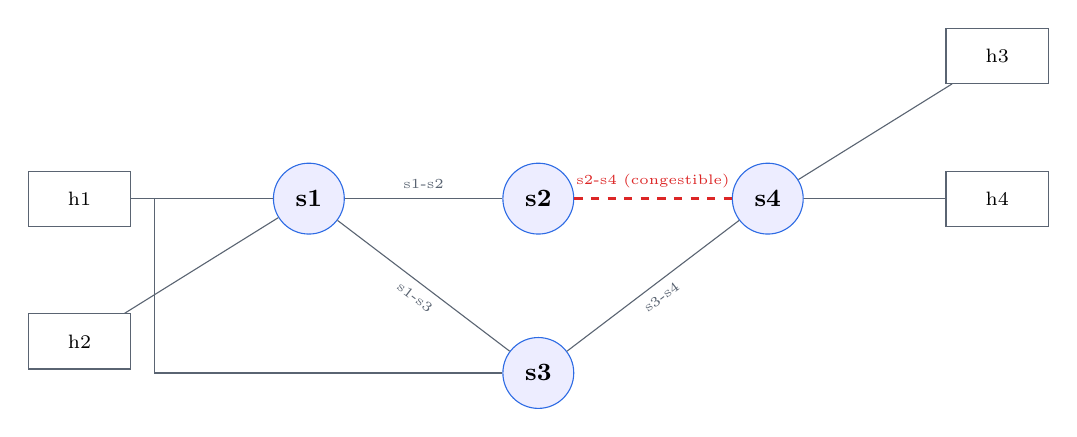
\begin{tikzpicture}[
    node distance=15mm and 16mm,
    sw/.style={circle, draw=sdnblue, fill=blue!7, minimum size=9mm, font=\small\bfseries, inner sep=0pt},
    host/.style={rectangle, draw=sdngrey, fill=white, minimum width=13mm, minimum height=7mm, font=\scriptsize, inner sep=1pt},
    cong/.style={draw=sdnred, very thick, dashed},
    norm/.style={draw=sdngrey},
    lbl/.style={font=\tiny, text=sdngrey}
]
\node[host] (h1) {h1};
\node[host] (h2) [below=11mm of h1] {h2};
\node[sw] (s1) [right=18mm of h1] {s1};
\node[sw] (s2) [right=20mm of s1] {s2};
\node[sw] (s4) [right=20mm of s2] {s4};
\node[sw] (s3) [below=13mm of s2] {s3};
\node[host] (h4) [right=18mm of s4] {h4};
\node[host] (h3) [above=11mm of h4] {h3};

\draw[norm] (h1) -- (s1);
\draw[norm] (h2) -- (s1);
\draw[norm] (h1.east) -- ++(3mm,0) |- (s3);
\draw[norm] (s1) -- node[lbl, above, sloped] {s1-s2} (s2);
\draw[cong] (s2) -- node[lbl, above, sloped, text=sdnred] {s2-s4 (congestible)} (s4);
\draw[norm] (s1) -- node[lbl, below, sloped] {s1-s3} (s3);
\draw[norm] (s3) -- node[lbl, below, sloped] {s3-s4} (s4);
\draw[norm] (s4) -- (h4);
\draw[norm] (h3) -- (s4);
\end{tikzpicture}
\end{center}

\begin{center}
\begin{tabular}{@{}L{3.6cm}L{9.4cm}@{}}
\toprule
\textbf{Element} & \textbf{Purpose} \\
\midrule
\texttt{h1 $\to$ h4} & The \emph{protected intent}: video flow that must stay under 50~ms. \\
\texttt{h3 $\to$ h4} & Voice flow, \emph{protected}: a recovery must not harm it. \\
\texttt{h2 $\to$ h3} & Congestion generator, forced over \texttt{s2-s4} by the shortest route. \\
\texttt{s2-s4} & The congestible link loaded by the scenario. \\
Ring \texttt{s1-s2-s4-s3-s1}
  & Gives two independent routes between source and sink --- \texttt{s1-s2-s4}
  at 10~ms and \texttt{s1-s3-s4} at 20~ms. This redundancy is what makes
  recovery possible at all. \\
\bottomrule
\end{tabular}
\end{center}

\subsection{The Demonstration Sequence}

\begin{enumerate}
    \item Start the lab, backend and dashboard; confirm a clean baseline.
    \item Press \textbf{Create Congestion}. The lab starts a UDP generator that
          loads \texttt{s2-s4}. The dashboard immediately shows the link in red
          and dashed, with utilisation climbing.
    \item Type \emph{``optimise latency so that it comes under 50 ms''} into the
          chat.
    \item Watch the agent gather evidence, pass the gates, and either reroute or
          explain why it did not.
\end{enumerate}

\subsection{What the Dashboard Shows}

Figure~\ref{fig:dashboard} is the live dashboard with the congestion scenario
active. The congested link is drawn in red and dashed with its live utilisation
labelled on the edge, and the link metrics table agrees with the picture.

\begin{figure}[H]
\centering
\includegraphics[width=\linewidth]{dashboard.png}
\caption{Live dashboard with the congestion scenario active on \texttt{s2-s4}.
The congested link renders red and dashed at 9\% utilisation, the link table
reports the same state, and the end-to-end chart plots live latency and packet
loss for the video flow.}
\label{fig:dashboard}
\end{figure}

\subsection{What the Agent Does}

Figure~\ref{fig:agent} shows the agent's response to the same prompt. Note the
trace: the intent is parsed, evidence is gathered and confirmed sufficient, and
the agent then reports \texttt{intent\_satisfied} with the measured figure. It
made no change, and said why.

\begin{figure}[htbp]
\centering
\includegraphics[width=\linewidth]{agent_run.png}
\caption{Agent run against the live lab. The transcript records intent
detection, the evidence verdict, and a terminal \texttt{intent\_satisfied}
outcome: measured latency was inside the 50~ms target, so no network change was
proposed.}
\label{fig:agent}
\end{figure}

% ============================ 6. EVALUATION ===============================
\section{Evaluation}

\subsection{Method}

All measurements were taken from the running lab through its snapshot endpoint,
which reads latency from ICMP ping inside the hosts and utilisation from the
switch port counters. Each phase was sampled five times and the mean reported.
The evaluation asks three questions:

\begin{enumerate}
    \item Does the congestion scenario produce \emph{real, observable} network
          change?
    \item When the network is healthy, does the agent correctly \emph{refuse to
          act}?
    \item When the network is genuinely violated, does it act correctly --- and
          does it report the outcome honestly?
\end{enumerate}

\subsection{Results}

\begin{center}
\begin{tabular}{@{}L{4.4cm}C{2.3cm}C{2.3cm}C{2.6cm}@{}}
\toprule
\textbf{Phase} & \textbf{Video} & \textbf{Peak} & \textbf{Loss} \\
 & \textbf{(mean)} & \textbf{(per flow)} & \textbf{(mean)} \\
\midrule
Baseline, no congestion       & 24.9~ms & 31.4~ms & 0.0\% \\
Congestion at 400~Mbps        & 26.7~ms & ---     & 0.0\% \\
Heavy overload                & 40.9~ms & 51.7~ms & 28.0\% \\
\bottomrule
\end{tabular}
\end{center}

Utilisation on the congested link tracked the offered load accurately up to
approximately 50~Mbps and then plateaued near 40~Mbps, which is the real
forwarding ceiling of the pure-Python switch rather than a measurement error.

\subsection{Interpretation}

\paragraph{The congestion scenario is real.}
Link utilisation rose from 0\% to approximately 9\% and the link's state changed
to congested, confirming that the traffic generator and the telemetry path both
function. An earlier revision of this project reported success while generating
no traffic at all, because the intended tool was not installed on the machine;
the failure was silent and the metrics stayed at zero. That class of silent
failure is precisely what this project exists to eliminate, so it is worth
noting that the scenario now reports failure if the generator does not start.

\paragraph{The agent correctly abstains on a healthy network.}
Against a 24.9~ms baseline with a 50~ms target, the agent returned
\texttt{intent\_satisfied} and made no change. This is the desired behaviour and
the most commonly mis-implemented one: a system that always finds something to
do is not reasoning, it is acting reflexively.

An important detail emerged during evaluation. An earlier revision compared only
the \emph{mean} of a flow's latency samples against the target. Under light
load a flow oscillated around the target, averaging 41.8~ms on a single reading
and so concluding ``satisfied'', while the dashboard simultaneously displayed a
breach. The check now evaluates the distribution of samples and treats a
sustained overrun as a violation, which is what a latency service-level
objective actually means.

\paragraph{The agent reroutes correctly under violation.}
Under heavy overload the intent was breached in five of five samples. The agent
identified the bottleneck, enumerated alternatives, and selected
\texttt{s1-s3-s4} --- the path that \emph{avoids} the congested \texttt{s2-s4}
link entirely, correctly rejecting the shorter 18~ms alternative that would have
routed straight back through the bottleneck. All nine safety checks passed and
the controller installed the rules.

\paragraph{The agent reports failure honestly.}
The reroute executed cleanly, and the verification gate then measured 51.6~ms
against the 50~ms target and returned \texttt{recovery\_failed} with the reason
stated plainly. This is the behaviour the whole design exists to produce. The
alternative --- reporting the successful command as a successful recovery ---
would have been indistinguishable from a working system to anyone reading the
audit log, and would have been wrong.

\subsection{Behaviour Under Uncertainty}

\begin{center}
\begin{tabular}{@{}L{4.6cm}L{8.4cm}@{}}
\toprule
\textbf{Condition} & \textbf{Observed behaviour} \\
\midrule
Intent already met
  & \texttt{intent\_satisfied}; no change; measurement quoted in the explanation. \\
Evidence missing or stale
  & \texttt{abstained\_insufficient\_evidence}; names the measurement it could
    not obtain. \\
All candidates rejected
  & Every rejection reported with its failing check. \\
Command executed, intent unmet
  & \texttt{recovery\_failed}; before and after measurements both recorded. \\
LLM unavailable
  & Deterministic parser used; the run states the model was not involved. \\
Lab unreachable
  & HTTP 503, never a blank but apparently healthy 200 response. \\
\bottomrule
\end{tabular}
\end{center}

\subsection{Testing}

\begin{center}
\begin{tabular}{@{}L{6.0cm}C{3.0cm}C{3.0cm}@{}}
\toprule
\textbf{Suite} & \textbf{Count} & \textbf{Result} \\
\midrule
Backend unit and integration   & 76 & pass \\
Frontend end-to-end (Playwright) & 4 & pass \\
Live lab (opt-in marker)       & 5 & available \\
\bottomrule
\end{tabular}
\end{center}

Regression tests are written for every defect discovered during development,
and each names the failure it prevents. Two examples that correspond directly to
the bugs described above:

\begin{itemize}
    \item \texttt{test\_samples\_over\_target\_are\_violated\_despite\_low\_mean}
          --- guards the mean-only comparison that produced a false
          \texttt{intent\_satisfied}.
    \item \texttt{test\_congestion\_free\_path\_outranks\_a\_faster\_congested\_one}
          --- guards the ranking that preferred an 18~ms detour through the
          bottleneck over the 20~ms path that avoided it.
\end{itemize}


% ============================ 7. PROGRESS STATUS =========================
\section{Current Status}\label{sec:status}

This is a progress report covering the work completed so far. The system described above is functional and running end to end.

\subsection{What Is Working}

\begin{itemize}
    \item A live Mininet/OpenFlow lab of four hosts and four switches, isolated
          in its own network namespace and driven by a Ryu controller.
    \item Continuous telemetry: per-flow latency and packet loss from ICMP, and
          per-link utilisation from switch port counters, streamed to the
          dashboard over Server-Sent Events.
    \item A working congestion scenario that generates real traffic and reports
          failure if the generator does not start.
    \item The complete agent graph with all three gates, verified against the
          running lab across healthy, violated and failed-recovery cases.
    \item 76 backend tests and 4 browser end-to-end tests, all passing.
\end{itemize}



\vfill
\begin{center}
\small\textit{All measurements in this report were taken from the running system
and are reproducible using the commands in the project README. Figures and
results reflect the state of the work at the time of submission and are
expected to change as the items above are completed.}
\end{center}

\end{document}